\section{Ablations: what the echo is actually made of}
\label{sec:ablations}

The diagnosis in Section~\ref{sec:background} makes a strong claim about what the
second image copy is for. It is not there to be re-perceived. It is there to put
image tokens after the question so the read-out step has something local to
attend to. That claim has a sharp consequence: the echoed copy should not need to
be legible. We test it by degrading the echo, by pricing it, and by asking
whether a prompt optimizer that can only edit text finds the same fix.

\subsection{The echoed copy does not need to be legible}
\label{sec:ablation-resolution}

We downscale only the second image occurrence in \sitit{}, leaving the first at
full resolution, and sweep the echo scale over $1$, $\tfrac{1}{2}$,
$\tfrac{1}{4}$ and $\tfrac{1}{8}$ (Table~\ref{tab:resolution}). On three of four
benchmarks a quarter-resolution echo matches or beats a full-resolution one:
POPE moves by $-0.05$ F1, Winoground by $+0.75$ group accuracy, and NaturalBench
by $+0.21$ pair accuracy.

Pushing to an eighth makes the point sharper. On NaturalBench, an echo carrying
$\tfrac{1}{64}$ of the original pixels scores $37.32$ group accuracy against the
full echo's $37.37$, a difference of $0.001$ with $p = 1.00$, while still beating
question-last by $+0.023$ ($p = 0.005$). The echo can be destroyed as an image
and keep its entire benefit.

RF20 is the exception, and it is the informative one. Its accuracy falls
monotonically as the echo degrades ($-0.50$ F1 at half, $-1.76$ at quarter).
RF20 asks whether a specific, often small object class is present in a
detection-style image, so the second look is doing real perceptual work there
rather than only re-anchoring. The split between RF20 and the other three says
the echo has two separable jobs, and that only one of them needs pixels.

\begin{figure}[t]
\begin{minipage}[t]{0.50\textwidth}
\vspace{0pt}
\centering
\captionof{table}{Echo-resolution sweep, Qwen3-VL-8B. Only the \emph{second}
image occurrence is downscaled; the first stays at full resolution. Three of four
benchmarks are flat or better at quarter resolution. RF20, whose targets are
small, degrades monotonically. Metrics are F1 for POPE and the RF20 presence task, group accuracy for Winoground, pair accuracy for NaturalBench. Blank cells were not run.}
\label{tab:resolution}
\vspace{2pt}
\small
\setlength{\tabcolsep}{3.5pt}
\begin{tabular}{lrrrr}
\toprule
Benchmark & Echo $1$ & $\tfrac{1}{2}$ & $\tfrac{1}{4}$ & $\tfrac{1}{8}$ \\
\midrule
POPE         & 88.12 & \best{88.35} & 88.07 & \\
Winoground   & 40.25 & \best{41.75} & 41.00 & \best{41.75} \\
NaturalBench & 80.36 & 80.55 & \best{80.57} & 80.18 \\
RF20 (presence) & \best{80.56} & 80.06 & 78.80 & \\
\bottomrule
\end{tabular}
\end{minipage}\hfill
\begin{minipage}[t]{0.47\textwidth}
\vspace{0pt}
\centering
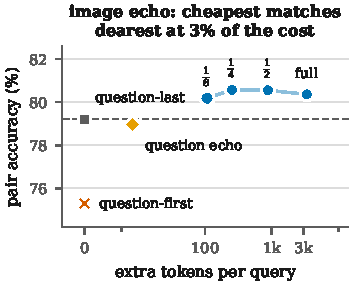
\includegraphics[width=\linewidth]{figs/fig_pareto.pdf}
\caption{Cost against accuracy on NaturalBench. The $x$ axis is extra tokens per
query versus question-first (symmetric log, so $0$ is shown); the dashed line is
question-last. Every image echo clears that baseline, and the
$\tfrac{1}{8}$-resolution echo ($+107$ tokens) is indistinguishable from the full
one ($+3{,}352$).}
\label{fig:pareto}
\end{minipage}
\end{figure}

\begin{finding}
\textbf{Finding.} The echoed image does not need to be legible. An
eighth-resolution echo, carrying $\tfrac{1}{64}$ of the pixels, is statistically
indistinguishable from a full-resolution one on NaturalBench ($37.32$ vs
$37.37$ group accuracy, $p = 1.00$) while still beating question-last
($p = 0.005$). Only RF20, whose targets are small, needs the pixels
($-1.76$ F1 at quarter resolution).
\end{finding}

\subsection{What echoing costs}
\label{sec:ablation-cost}

Prompt-level interventions are usually reported without their bill. We count
exact token counts for each ordering with the Qwen3-VL-8B processor over 20
images spanning RF20's constituent datasets, separating vision from text tokens
(Table~\ref{tab:cost} in Appendix~\ref{app:cost}).

The two echo mechanisms are three orders of magnitude apart. Repeating the
question costs $13$ tokens. Repeating the image at full resolution costs
$3{,}352$, which roughly doubles the prompt. Downscaling the echo collapses that
cost quickly, because vision-token count falls with area: a half-resolution echo
costs $875$ added tokens, a quarter-resolution echo $252$, and an
eighth-resolution echo $107$. Figure~\ref{fig:pareto} puts the two axes
together. The accuracy curve is flat across a $31\times$ range of echo cost, so
the operating point to ship is the cheapest one.


\begin{finding}
\textbf{Finding.} Echo cost is a tunable knob, not a fixed doubling of the
prompt. A full-resolution image echo adds $3{,}352$ tokens per query, but a
quarter-resolution echo adds $252$ ($7.5\%$) and an eighth-resolution echo adds
$107$ ($3.2\%$) for indistinguishable accuracy, while question echoing adds $13$.
\end{finding}

\subsection{Prompt optimization finds part of the fix, and only where the
mechanism says it should}
\label{sec:ablation-gepa}
\label{sec:gepa}

A reviewer will reasonably ask whether careful prompt engineering would do the
same work as echoing, making the ordering story incidental. We test this with
GEPA \citep{gepa2025}, a reflective prompt optimizer, and use it as a prediction
test rather than as a baseline to beat.

The mechanism predicts an asymmetry. GEPA may rewrite the system message text
but cannot move the image, so it cannot repair a read-out failure caused by
token order. It should find recoverable headroom under \sti{}, where read-out is
broken, and little or nothing under \sit{}, where it is not. That is what
happens (Table~\ref{tab:gepa}, Appendix~\ref{app:gepa}). Under \sti{}, GEPA
improves all three benchmarks: POPE $86.41 \to 87.25$, VQAv2 $86.11 \to 88.13$,
NaturalBench $74.74 \to 75.79$. Under \sit{}, the same optimizer with the same
budget returns the seed prompt unchanged on POPE and VQAv2, both exact ties, and
regresses NaturalBench by $0.41$ by overfitting its validation split.

Two further numbers matter. First, \sit{}'s baseline is higher than \sti{}'s on
every benchmark ($88.27$ vs $86.41$, $88.55$ vs $86.11$, $78.80$ vs $74.74$),
so the asymmetry is a headroom effect and not a quirk of the optimizer. Second,
GEPA's best \sti{} prompt never reaches the plain \sit{} baseline: it closes
$26\%$ to $83\%$ of the \sti{}-to-\sit{} gap and stops there. Its optimized
prompts add $26$, $32$ and $71$ tokens per query, less than even an
eighth-resolution echo, but its search costs $157{,}725$ to $982{,}343$ tokens
once plus a separate reflection model. Rewording the prompt recovers part of
what bad ordering costs. Moving or echoing the image recovers the rest.

\begin{table}[t]
\caption{GEPA prompt optimization under two orderings, Qwen3-VL-8B, on held-out
evaluation sets. GEPA finds real gains under \sti{} and nothing under \sit{},
as the read-out diagnosis predicts. It never reaches the \sit{} baseline it is
competing with.}
\label{tab:gepa}
\begin{center}
\small
\setlength{\tabcolsep}{4pt}
\begin{tabular}{llrrrrr}
\toprule
 & & & \multicolumn{2}{c}{Accuracy} & & Gap \\
\cmidrule(lr){4-5}
Benchmark & Order & $N$ & Seed & GEPA & $\Delta$ & closed \\
\midrule
\multirow{2}{*}{POPE}         & \sti{} & 8{,}800 & 86.41 & 87.25 & $+0.84$ & $45\%$ \\
                              & \sit{} & 8{,}800 & 88.27 & 88.27 & $+0.00$ & n/a \\
\midrule
\multirow{2}{*}{VQAv2}        & \sti{} & 10{,}000 & 86.11 & 88.13 & $+2.02$ & $83\%$ \\
                              & \sit{} & 10{,}000 & 88.55 & 88.55 & $+0.00$ & n/a \\
\midrule
\multirow{2}{*}{NaturalBench} & \sti{} & 7{,}000 & 74.74 & 75.79 & $+1.04$ & $26\%$ \\
                              & \sit{} & 7{,}000 & 78.80 & 78.39 & $-0.41$ & n/a \\
\bottomrule
\end{tabular}
\end{center}
\end{table}

\begin{finding}
\textbf{Finding.} Prompt optimization behaves exactly as the read-out diagnosis
predicts: GEPA gains under \sti{} (POPE $+0.84$, VQAv2 $+2.02$, NaturalBench
$+1.04$) and finds nothing under \sit{} (two exact ties and $-0.41$), because
\sit{} has less headroom to recover. It closes $26\%$ to $83\%$ of the
\sti{}-to-\sit{} gap and never reaches the \sit{} baseline, so rewording is not
a substitute for fixing token order.
\end{finding}
